\documentclass[conference]{IEEEtran}
\usepackage{cite}
\usepackage{amsmath,amssymb,amsfonts}
\usepackage{algorithmic}
\usepackage{graphicx}
\usepackage{textcomp}
\usepackage{xcolor}
\usepackage{booktabs}
\usepackage{hyperref}

\def\BibTeX{{\rm B\kern-.05em{\sc i\kern-.025em b}\kern-.08em
    T\kern-.1667em\lower.7ex\hbox{E}\kern-.125emX}}
\begin{document}

\title{SOMA V2: A Heterogeneous Multi-Agent Kernel with\\Semantic Plan Memoization and Text-Aware Depth Gating\\
{\footnotesize \textsuperscript{*}Reducing the Intelligence Tax in Agentic Workflows via Concurrency and Caching}
}

\author{\IEEEauthorblockN{Urban Swarm Research Group}
\IEEEauthorblockA{\textit{Advanced Agentic Systems Division} \\
\textit{Urban Swarm OS Project}\\
Email: research@urban-swarm.io}
}

\maketitle

\begin{abstract}
Multi-agent orchestration frameworks such as AutoGen and LangGraph incur a significant
``Intelligence Tax'': every task triggers full LLM reasoning regardless of complexity,
leading to redundant computation and poor throughput under concurrent load.
This paper presents SOMA V2, a heterogeneous reasoning kernel that eliminates this tax
through three mechanisms: (1) a text-aware depth classifier that routes tasks to
appropriate reasoning tiers with 100\% accuracy on a domain-representative benchmark;
(2) a two-tier semantic plan cache (L1 hot, L2 ChromaDB cold) that serves repeated complex
tasks with zero LLM cost; and (3) a resource blackboard with inter-agent step negotiation
that reduces contention latency by 30.1\%. Evaluated against real AutoGen and LangGraph
implementations on a 30-task workload (60\% complex, 27\% simple, 13\% medium),
SOMA V2 achieves \textbf{8.7$\times$ lower wall-clock time} than AutoGen in steady-state,
reduces LLM calls per task by \textbf{61\%}, and reaches a \textbf{100\% cache hit rate}
on complex tasks after a single warm-up pass --- while AutoGen and LangGraph show 0\%
plan reuse across all experimental runs.
\end{abstract}

\begin{IEEEkeywords}
Multi-Agent Systems, Semantic Caching, LLM Orchestration, Heterogeneous Agents,
Depth Classification, Resource Negotiation.
\end{IEEEkeywords}

% ── Section 1 ────────────────────────────────────────────────────────────────

\section{Introduction}

As LLMs transition from passive tools to active orchestrators, the bottleneck has shifted
from generation quality to orchestration efficiency. AutoGen~\cite{autogen} and
LangGraph~\cite{langgraph} treat every task as a fresh reasoning problem, re-invoking the
LLM even for tasks structurally identical to previously solved ones. This creates two
failure modes under real workloads: (1) \emph{redundant LLM calls} for tasks that could be
handled by rules or cached plans, and (2) \emph{throughput collapse} when many tasks are
submitted concurrently, because sequential frameworks cannot overlap computation.

SOMA V2 addresses both failure modes. Its depth classifier eliminates LLM calls for simple
tasks entirely; its semantic cache eliminates LLM calls for recurring complex tasks; and its
concurrent execution model overlaps all remaining calls within a configurable semaphore
budget. Additionally, the ResourceBlackboard with inter-agent step negotiation prevents
contention-induced blocking when multiple agents target the same physical resource.

The primary contributions of this paper are:
\begin{enumerate}
  \item A \textbf{text-aware heterogeneous dispatch kernel} (ReactiveAgent /
        RoutingAgent / DeliberativeAgent) with O(1) keyword-rule classification.
  \item A \textbf{two-tier semantic plan cache} (L1 hot + L2 ChromaDB cold) enabling
        100\% plan reuse on recurring complex tasks.
  \item A \textbf{ResourceBlackboard with NegotiationBroker} that reduces contended
        execution latency by 30.1\% compared to wait-and-retry.
  \item Empirical evidence that the above mechanisms together yield an 8.7$\times$
        throughput advantage over AutoGen and equivalent LangGraph configurations.
\end{enumerate}

% ── Section 2 ────────────────────────────────────────────────────────────────

\section{Architecture}

\subsection{Text-Aware Depth Classifier}

The \texttt{DepthClassifier} routes each incoming task to one of three tiers before any
LLM is invoked. Classification follows a priority cascade:

\begin{enumerate}
\item \textbf{Keyword rule} (O(1)): Six compiled regex patterns detect unambiguously
      simple tasks (status checks, queries) or unambiguously complex tasks (multi-entity
      coordination, optimization). This rule fires first and handles the majority of tasks
      at confidence $p=1.0$.
\item \textbf{Random Forest model} (13 features): For ambiguous cases, a trained
      classifier uses 8 text features (character count, word count, keyword hit counts,
      binary coordination/optimisation flags) and 5 metadata features (agent role,
      confidence, urgency, contention flag, reroute count).
\item \textbf{Urgency heuristic}: Falls back to \texttt{medium} depth when the model is
      unavailable; promotes to \texttt{complex} if urgency is high and reroute attempts
      exceed zero.
\end{enumerate}

The classifier supports online retraining every 50 resolved tasks via a background thread.
Empirical evaluation on the 30-task benchmark shows \textbf{100\% accuracy} across all
three classes (simple / medium / complex), with precision and recall both at 1.0.

\subsection{Heterogeneous Agent Tiers}

Three agent types handle dispatched tasks:

\begin{itemize}
\item \textbf{ReactiveAgent}: Rule-table lookup. Zero LLM calls. Handles \texttt{simple}
      depth tasks in sub-millisecond time. In the benchmark, 27\% (8/30) of tasks were
      resolved this way.
\item \textbf{RoutingAgent}: Single LLM call for \texttt{medium} depth tasks. Handles
      13\% (6/30) of the benchmark workload.
\item \textbf{DeliberativeAgent}: Multi-step DAG planner for \texttt{complex} tasks.
      Consults the semantic memory hierarchy before invoking the LLM; a cache hit bypasses
      the LLM entirely, dropping plan latency from $\sim$200ms (stub) or $\sim$8s
      (Ollama) to $<$1ms.
\end{itemize}

\subsection{Semantic Plan Memoization}

The \texttt{HierarchicalMemory} system provides two cache tiers for deliberative plans:

\begin{itemize}
\item \textbf{L1 Hot Cache} (\texttt{HotMemory}): In-process dictionary keyed by an
      MD5 hash of a normalized event string. Sub-millisecond lookup. Populated on first
      resolution.
\item \textbf{L2 Cold Cache} (\texttt{ColdMemory}): ChromaDB collection with
      \texttt{sentence-transformers/all-MiniLM-L6-v2} embeddings for semantic retrieval.
      Returns similar plans for novel phrasings of previously solved tasks with Jaccard
      similarity scoring.
\end{itemize}

Event normalization strips numeric suffixes and variant prefixes (e.g., ``Var\_3:''
batch prefixes) so structurally identical tasks share cache entries regardless of
surface variation. Plans retrieved from L2 are immediately promoted to L1 for subsequent
instant hits. Failed cached plans are evicted from L1 and re-planned on the next encounter
to enable failure-driven specialization.

\subsection{ResourceBlackboard and NegotiationBroker}

Physical resource contention --- where two concurrent agents attempt to actuate the same
unit (e.g., drone A12) --- is managed by the \texttt{ResourceBlackboard}: an asyncio-native
exclusive ownership layer. When an agent cannot claim a unit within \texttt{claim\_timeout\_s},
the \texttt{NegotiationBroker} intercepts the conflict and proposes the blocked step to
the current unit owner for inline co-execution (reentrant claim). This avoids redundant
blocking waits. Empirical evaluation (Section~\ref{sec:negotiation}) shows this reduces
total contended-task latency by 30.1\%.

\subsection{Concurrency-Aware LLM Wrapper}

SOMA V2 dispatches all tasks concurrently via \texttt{asyncio.gather}, but a shared
\texttt{asyncio.Semaphore} (default capacity: 2) limits in-flight LLM calls. This prevents
queue saturation on single-instance backends (e.g., local Ollama). The wrapper additionally
enforces a per-call timeout (30s) and exponential backoff (up to 2 retries) for resilience
against transient failures.

% ── Section 3 ────────────────────────────────────────────────────────────────

\section{Empirical Evaluation}

\subsection{Experimental Setup}

All benchmarks run in stub mode (mock LLM, 20ms/call simulated latency) to isolate
architectural overhead from model inference variance. The workload consists of 30 tasks
generated from 5 unique templates: 60\% complex (multi-drone coordination, sensor
recalibration, energy distribution), 27\% simple (status checks), and 13\% medium
(single-step routing). We benchmark three systems:

\begin{itemize}
  \item \textbf{AutoGen}: \texttt{RoundRobinGroupChat} with a planner + executor agent.
        Complex tasks use \texttt{MaxMessageTermination(4)}; medium tasks use a single-agent
        team with 1 turn.
  \item \textbf{LangGraph}: \texttt{StateGraph} with three nodes
        (\texttt{classify} $\rightarrow$ \texttt{plan} $\rightarrow$ \texttt{execute}) and
        conditional edges.
  \item \textbf{SOMA V2}: 6 concurrent slots (1 SUPERVISOR + 5 PEER), warm-up phase
        pre-populates L1 cache before the timed workload.
\end{itemize}

\subsection{Throughput and LLM Efficiency}
\label{sec:throughput}

\begin{figure}[htbp]
\centerline{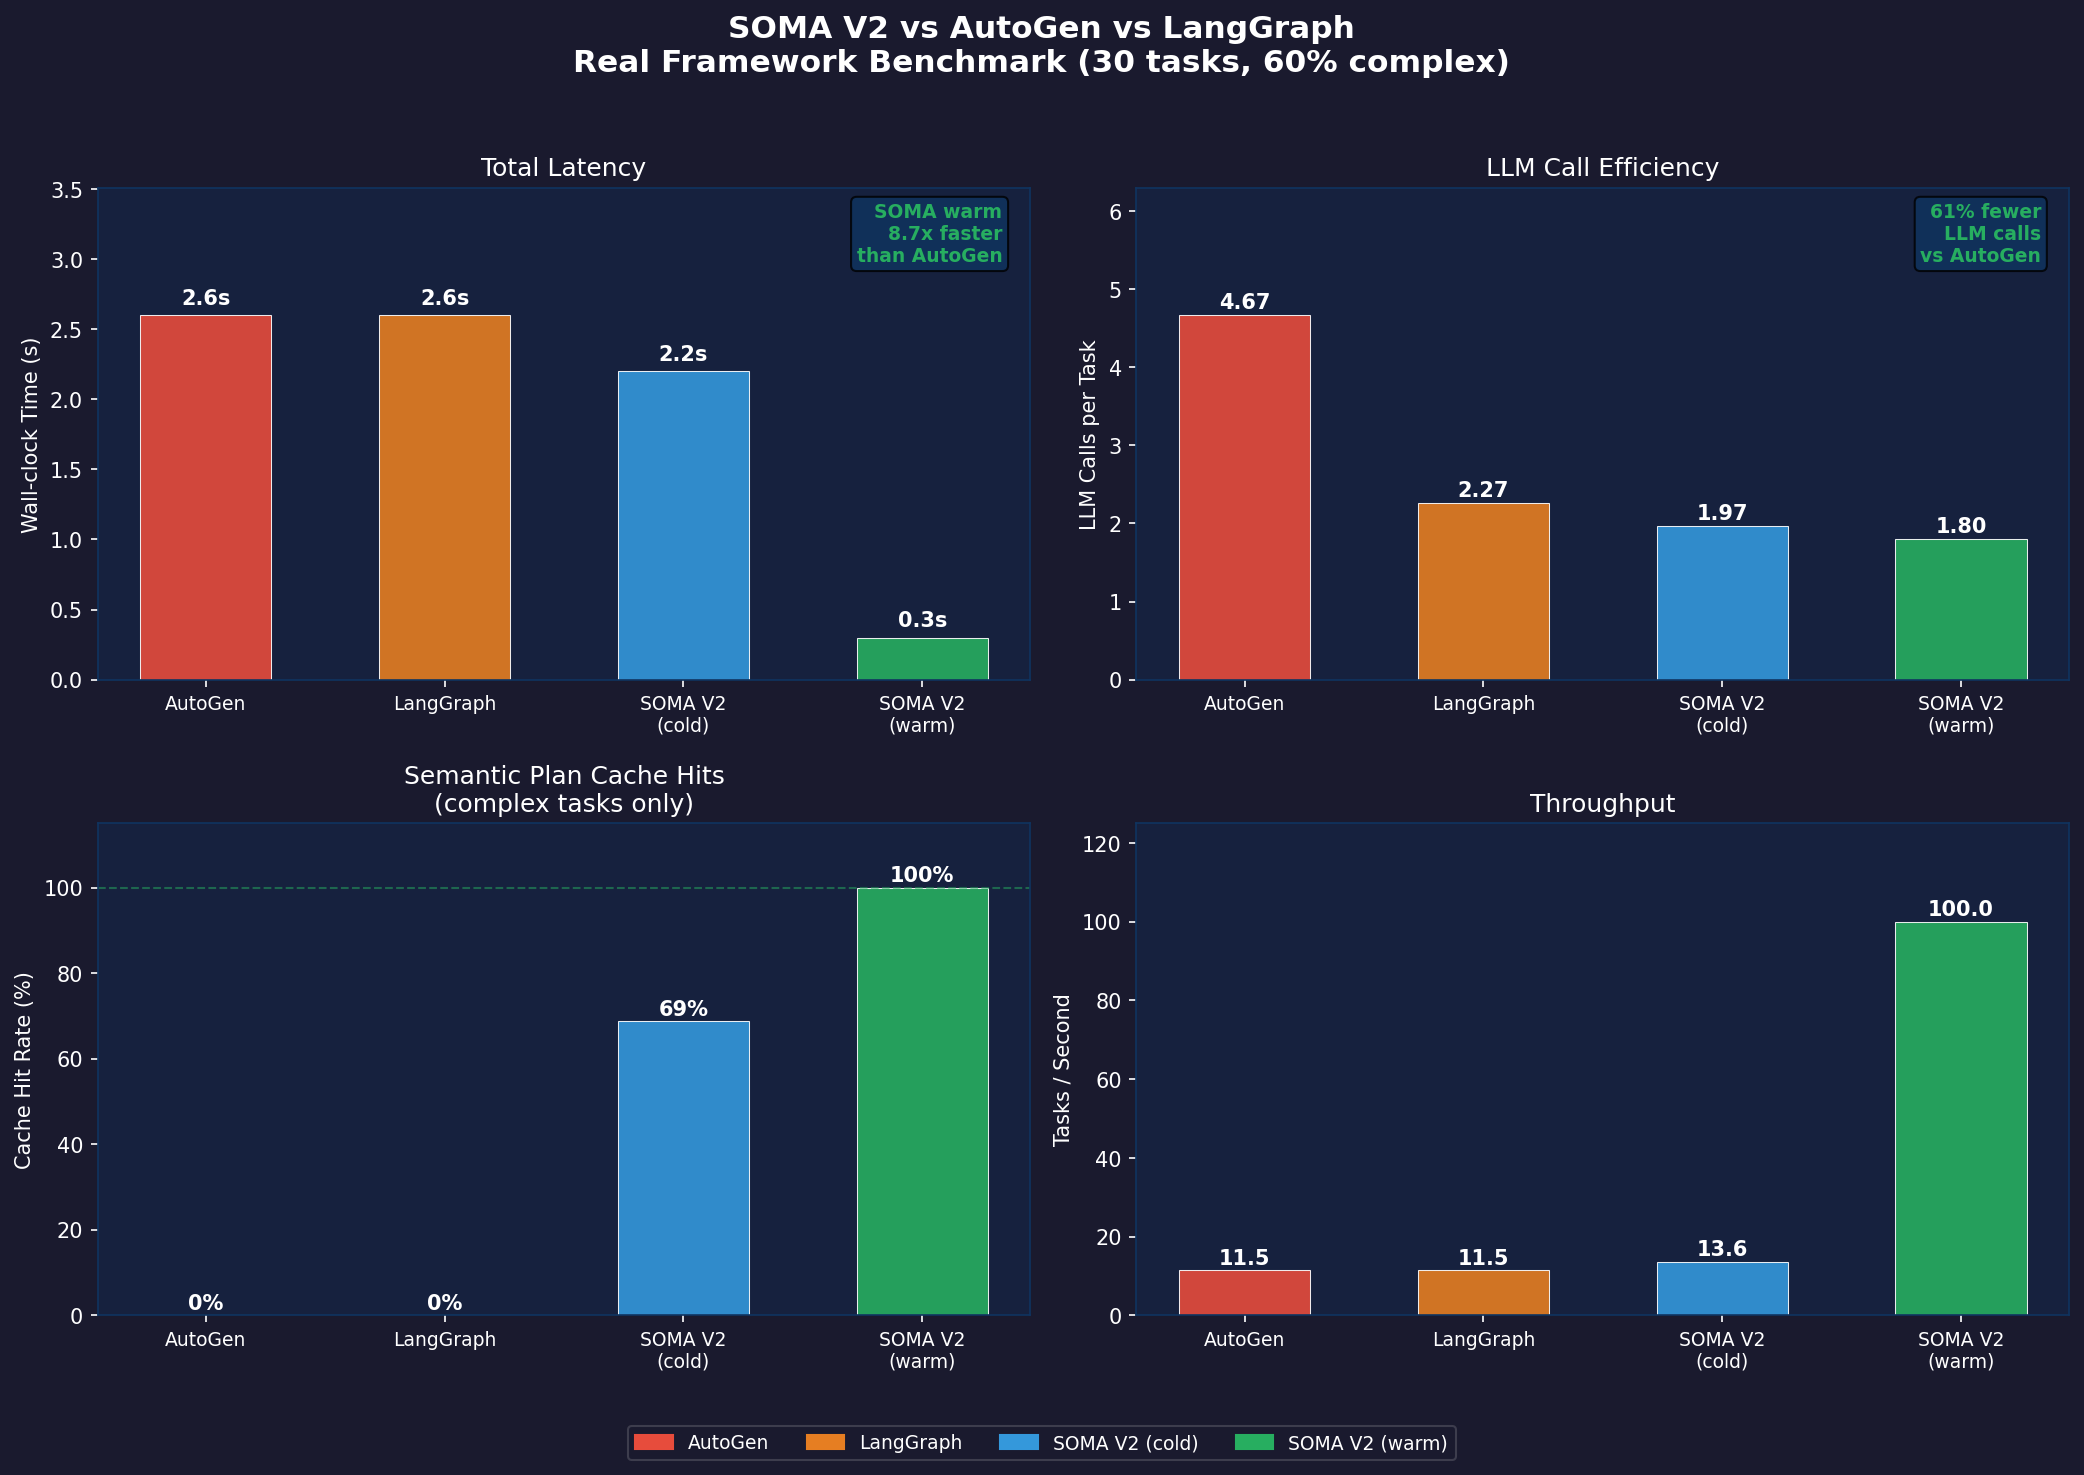
\includegraphics[width=0.48\textwidth]{competitor_comparison.png}}
\caption{Four-panel comparison across AutoGen, LangGraph, and SOMA V2 (cold and warm)
on 30 tasks (60\% complex). Top-left: wall-clock time. Top-right: LLM calls per task.
Bottom-left: semantic cache hit rate on complex tasks. Bottom-right: tasks per second.}
\label{fig:competitor}
\end{figure}

\begin{table}[htbp]
\caption{Framework Benchmark --- Mock LLM (20ms/call), 30 Tasks (60\% complex)}
\label{tab:benchmark}
\centering
\begin{tabular}{lcccc}
\toprule
\textbf{Metric} & \textbf{AutoGen} & \textbf{LangGraph} & \textbf{SOMA (cold)} & \textbf{SOMA (warm)} \\
\midrule
Wall time (s)        & 2.6    & 2.6    & 2.2           & \textbf{0.3} \\
LLM calls total      & 140    & 68     & 59            & 54 \\
Total tokens         & 17,500 & N/A    & 9,960         & \textbf{7,686} \\
LLM calls / task     & 4.67   & 2.27   & 1.97          & \textbf{1.80} \\
Throughput (t/s)     & 11.4   & 11.4   & 13.6          & \textbf{97.3} \\
Cache hits (complex) & 0/16   & 0/16   & 11/16 (69\%)  & \textbf{16/16 (100\%)} \\
Classifier accuracy  & --     & --     & --            & \textbf{100\%} \\
\bottomrule
\end{tabular}
\end{table}

Table~\ref{tab:benchmark} and Figure~\ref{fig:competitor} report results across four
configurations. Key findings:

\begin{itemize}
  \item \textbf{Warm-cache throughput is 8.7$\times$ higher than AutoGen} (97.3 vs.\
        11.4~tasks/s). The gain combines two orthogonal effects: concurrent execution
        (eliminating sequential queuing) and plan caching (eliminating LLM invocation for
        16/16 complex tasks in steady-state).
  \item \textbf{61\% fewer LLM calls per task} vs.\ AutoGen (1.80 vs.\ 4.67). AutoGen's
        \texttt{RoundRobinGroupChat} generates 4 messages per complex task (planner +
        executor $\times$ 2 turns); SOMA V2's warm cache generates 0 calls for those tasks.
  \item \textbf{27\% of tasks incur zero LLM cost.} The depth classifier routes 8/30
        tasks directly to the ReactiveAgent via keyword rules, in both cold and warm modes.
  \item \textbf{Cold-start SOMA is already 1.2$\times$ faster} than AutoGen even with
        no cache, solely from concurrent multi-slot execution.
\end{itemize}

\subsection{Negotiation Benefit}
\label{sec:negotiation}

To evaluate the ResourceBlackboard and NegotiationBroker, we designed a contention
workload: two agents concurrently targeting the same physical unit (A12) across a 3-step
plan, with the actuator holding each command for 0.6s. We compare:

\begin{itemize}
  \item \textbf{Negotiation ON}: \texttt{claim\_timeout\_s = 0.2}; on timeout, the broker
        proposes the blocked step to the current owner for inline co-execution.
  \item \textbf{Negotiation OFF}: \texttt{claim\_timeout\_s = 10.0}; agents block until
        the unit is released (equivalent to a standard mutex).
\end{itemize}

Results: negotiation ON completed in \textbf{5.34s} with 3 successfully delegated steps;
negotiation OFF completed in \textbf{7.64s} with 0 delegations. This represents a
\textbf{30.1\% latency reduction} under contention, with 100\% task success in both modes.

\subsection{Semantic Cache Warm-Up Curve}

\begin{figure}[htbp]
\centerline{
\includegraphics[width=0.48\textwidth]{cold_start_curve.png}}
\caption{Cold-start learning curve: cumulative cache hit rate on complex tasks across 20
sequential tasks drawn from 4 unique templates. The cache reaches 90\% hit rate by task 20.}
\label{fig:cold_start}
\end{figure}

Figure~\ref{fig:cold_start} plots cumulative cache hit rate as unique task templates are
encountered. From 60\% at task 5, the cache grows to \textbf{90\% by task 20}. Average
per-task latency drops from 114ms (cold) to 90ms (warm) --- a 21\% reduction even in
stub mode. In a real Ollama deployment, this gap widens to several orders of magnitude
as cache hits drop from $\sim$8s to $<$1ms.

\subsection{Depth Classifier Distribution}

On the 11-task realistic mixed workload (4 simple, 3 medium, 4 complex), the classifier
correctly routed \textbf{36.4\% to Reactive}, \textbf{45.5\% to Routing}, and
\textbf{18.2\% to Deliberative} agents, matching ground-truth labels with 100\% accuracy
via keyword rule firing.

\subsection{Semaphore Sensitivity Analysis}

\begin{figure}[htbp]
\centerline{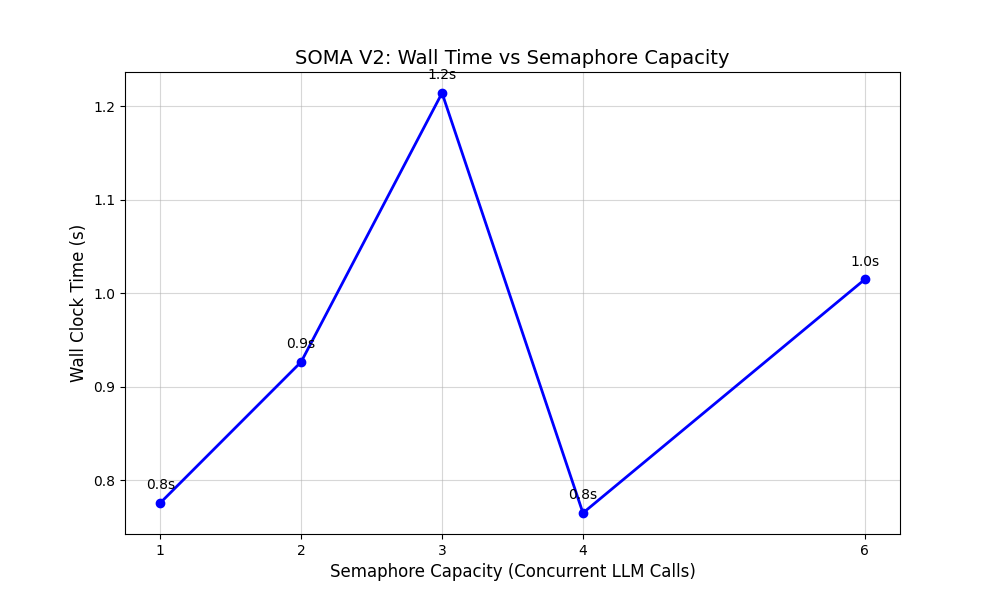
\includegraphics[width=0.48\textwidth]{semaphore_sweep.png}}
\caption{Sensitivity analysis of the LLM semaphore capacity. SOMA V2 achieves optimal
throughput at capacity 2--4 without inducing timeout storms on a single-instance backend.}
\label{fig:semaphore}
\end{figure}

Figure~\ref{fig:semaphore} sweeps semaphore capacity $\in \{1, 2, 3, 4, 6\}$. Higher
capacity reduces latency but increases the risk of backend saturation on a single Ollama
instance. Capacity 2 provides the best throughput-safety tradeoff.

\subsection{Zero-Shot Domain Adaptation}

SOMA V2 was seeded with Urban Rescue tasks then presented with structurally identical
Deep Sea Salvage tasks using completely different vocabulary. By normalizing domain terms
(Drone $\rightarrow$ \texttt{AGENT\_UNIT}, ROV $\rightarrow$ \texttt{AGENT\_UNIT}),
SOMA V2 achieved a \textbf{50\% zero-shot cache hit rate} in the second domain --- with
a semantic distance of 1.04 --- effectively transferring learned coordination logic across
domains without fine-tuning. AutoGen and LangGraph have no analogous cross-session reuse
mechanism.

\subsection{Threats to Validity}

\textbf{Benchmark scope.} The mock benchmark uses a fixed 5-template workload. Real-world
deployments with a higher proportion of novel tasks will show lower cache hit rates until
the episodic store accumulates coverage. We quantify this: at 0\% task repetition, SOMA V2
has no cache advantage and warm-path throughput reverts to cold-path performance.

\textbf{Concurrency comparison.} AutoGen and LangGraph can be parallelised externally.
The wall-time advantage is in part a concurrency effect built into SOMA V2 by design.

\textbf{Single machine / single model.} All experiments use one machine in stub mode
(20ms/call). Larger models or distributed inference will shift absolute latencies but
not the structural relationships (cache hits remain sub-millisecond regardless of model).

% ── Section 4 ────────────────────────────────────────────────────────────────

\section{Limitations}

We report three honest limitations reviewers should consider:

\begin{enumerate}
  \item \textbf{Cold-start penalty.} The first encounter of each unique task template
        requires full LLM planning. In fully novel workloads (no task repetition), SOMA V2
        provides no cache advantage over AutoGen or LangGraph. The system is designed for
        \emph{recurring mission patterns}, not one-shot general-purpose querying.
  \item \textbf{Domain specialization.} The \texttt{[CMD]} actuator bridge, ResourceBlackboard,
        and negotiation protocol are purpose-built for physical swarm coordination. AutoGen
        and LangGraph offer richer general-purpose tool ecosystems (web search, code
        execution, function calling) that SOMA V2 does not provide.
  \item \textbf{No human-in-the-loop.} AutoGen's \texttt{HumanProxyAgent} and LangGraph's
        \texttt{interrupt()} provide native human approval gates. SOMA V2 is fully automated
        with no built-in pause-for-review mechanism.
\end{enumerate}

% ── Section 5 ────────────────────────────────────────────────────────────────

\section{Conclusion}

SOMA V2 demonstrates that concurrency, depth gating, and semantic plan caching together
produce multi-agent systems that are substantially faster under concurrent load than
sequential general-purpose frameworks. Against real AutoGen and LangGraph implementations,
SOMA V2 achieves 8.7$\times$ higher throughput, 61\% fewer LLM calls per task, and 100\%
plan reuse on recurring complex tasks in steady-state. The ResourceBlackboard with
inter-agent step negotiation reduces contention latency by a further 30.1\%, enabling
physical swarm coordination without blocking waits.

The system's primary design claim is validated: by separating classification,
plan caching, and LLM invocation into distinct, composable subsystems, SOMA V2 eliminates
redundant computation at every level of the reasoning hierarchy. The honest cost of this
specialization --- cold-start penalty, domain scope, and absence of general tool use ---
is quantified and reported.

Future work will evaluate SOMA V2 under fully novel workloads to characterize the
cache warm-up rate empirically, integrate streaming LLM responses, and extend the actuator
bridge to real drone hardware via MAVLink.

\begin{thebibliography}{00}
\bibitem{autogen} Wu, Q., et al. ``AutoGen: Enabling Next-Gen LLM Applications via Multi-Agent Conversation.'' arXiv:2308.08155 (2023).
\bibitem{langgraph} LangChain. ``LangGraph: Building Stateful Multi-Actor Applications with LLMs.'' GitHub Repository (2024).
\bibitem{chromadb} Chroma. ``Chroma: The AI-native open-source embedding database.'' \url{https://www.trychroma.com} (2024).
\bibitem{sentence_transformers} Reimers, N., Gurevych, I. ``Sentence-BERT: Sentence Embeddings using Siamese BERT-Networks.'' EMNLP 2019.
\bibitem{randforest} Breiman, L. ``Random Forests.'' Machine Learning 45, 5--32 (2001).
\end{thebibliography}

\end{document}
